\section{Entwicklung des Honeynets}
Es gibt zwei verschieden Arten von Architekturen die sich im Laufe der Zeit durchgesetzt haben. Diese werden in Generation I und Generation II Honeynets (Abk. GenI und GenII) unterteilt.\\
\\
Bei einem GenI Honeypot wird das gesamte Netz durch eine Firewall in drei Teile unterteilt. Der erste Teil ist das Produktivnetz indem sich das zentrale Management System befindet. Der zweite Teil ist das Internet, welcher das Zugangsmedium des Angreifers darstellt. Der dritte und letzte Teil ist das Honeynet. 

Der Prozess der Datensammlung beginnt bereits mit passieren der Firewall. Dort können Informationen wie die verwendeten Protokolle, Zeitstempel,IP-Adressen und Ports gesammelt werden. Außerdem wird hier kontrolliert wie oft der Angreifer eine Verbindung eingehen kann (Data Control). Wie viele Versuche zugelassen werden hängt vom Verwendungszweck des Honeynets ab. Der Router zwischen Honeynet und Firewall unterstützt diese auf zwei verschiedene weisen. Zum Einem versteckt er die Firewall vor dem Hacker. Der Angreifer denkt, er greift auf einen produktiven Router zu. Zum Anderen unterstützt er die Firewall in Sachen Zugriffskontrolle. So kann ein Single-Point-of-Failure vermieden werden. 

Ein IDS-System steht nun noch zwischen dem Angreifer und den Honeypots. Dieses ist meist über einen Switch (oder wie in Abb. \ref{hnet:geni} mit einem Router) mit dem gesamten Honeynet verbunden. Dort werden alle Netzwerkaktivitäten protokolliert und bei bestimmten Angriffsmustern gegebenenfalls ein Alarm ausgelöst. 
\\
\begin{figure}[ht]
    \centering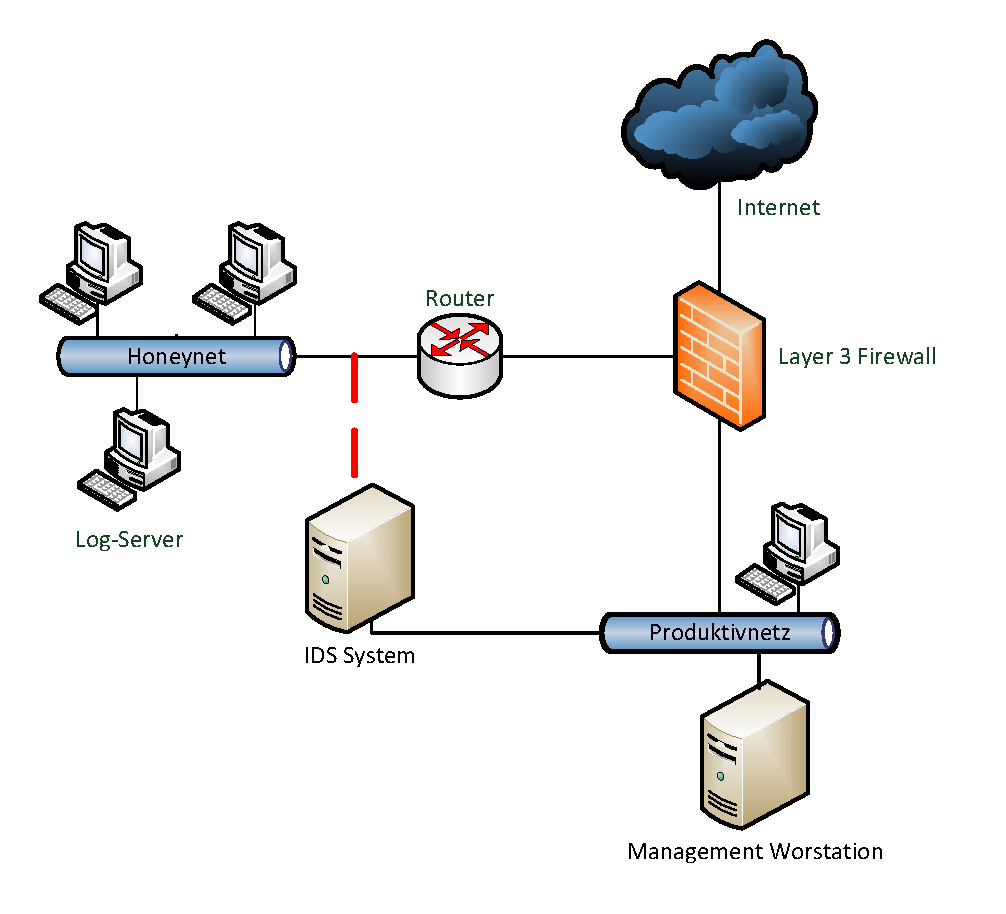
\includegraphics[scale=0.5]{Bilder/GenI.pdf}
  \caption{GenI Honeynet}
  \label{hnet:geni}
\end{figure}
\\
Nun kann der Angreifer auf die Honeypots direkt zugreifen. Auf diesen werden die genauen System-spezifischen Aktionen protokolliert.\\
\\
Die zweite Generation von Honeynets verwendet ein Gateway, welches die Funktionen der in GenI verwendetet Komponenten enthält, und diese noch weiter ergänzt. Dieses Gateway (meist Honeywall genannt) besteht nicht wie in GenI aus einem Layer-3 Router sondern aus einer Layer-2 Bridge. Dies verhindert z.B. dass der Angreifer über die TTL-Zähler eines IP-Paketes dn Router erkennen würde. Alle zuvor genannten Anforderungen werden in der Honeywall erfüllt. Für die Datenkontrolle werden hier wie in GenI die Verbindungen limitiert (oft mit dem Programm IPTables), um so DOS-Angriffe zu vermeiden und die Kontrolle über die Verbindungen zu erhalten. Zusätzlich bietet sich nun auch die Möglichkeit Zugriffe die über bestimmte Protokolle einzeln zu limitieren.

Ein IDS oder IPS verhindert weiterhin das der Hacker vom Honeynet aus einen Angriff auf das Produktivsystem oder in das Internet starten kann. Die Zugriffskontrolle und das IDS sammeln wie beim GenI Honeypot die Daten. In Abb. \ref{hnet:genii} befindet sich ein Beispiel einer GenII Honeynet Architektur.
\\
\begin{figure}[]
    \centering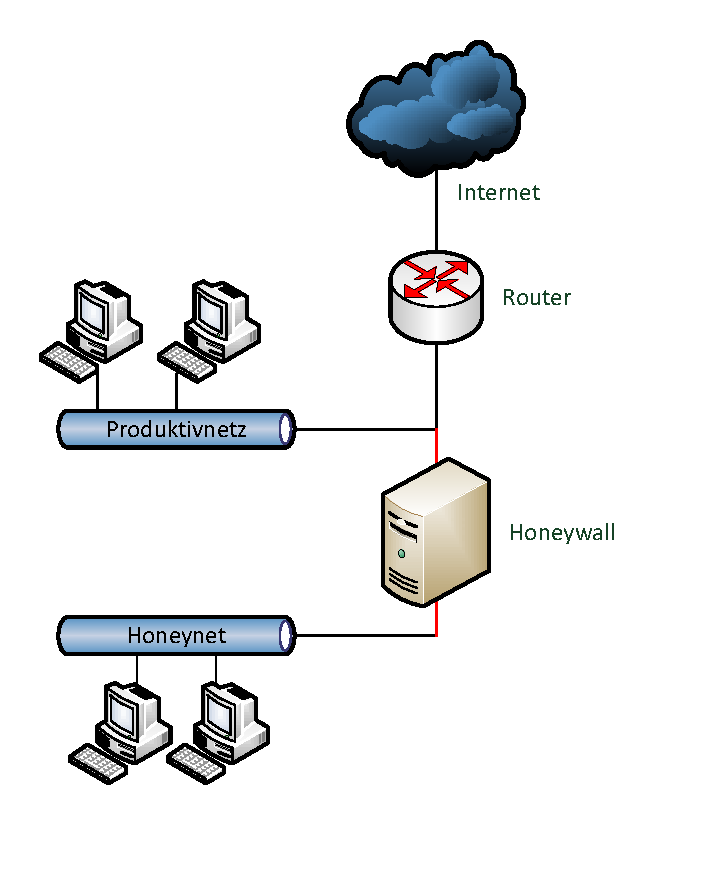
\includegraphics[scale=0.5]{Bilder/GenII.pdf}
  \caption{GenII Honeynet}
  \label{hnet:genii}
\end{figure}
\\
\noindent Ende 2004 wurde die vorerst letzte Generation von Honeynets vorgestellt. Ein GenIII Honeynet besitzt die selbe Netzwerkarchitektur wie dessen Vorgänger, behebt jedoch einig dessen Schwachstellen. Bei dem Versuch einen Honeynet Standard und eine Möglichkeit zu finden, ein Honeynet leichter zu Erstellen, veröffentlichte das Honeynet-Project (www.honeynet-project.org) eine CD, die alle Anforderungen eines Honeynets beinhaltet. Diese CD (\emph{Roo} genannt) wird als dritte Generation angesehen. Die aktuelle Version (1.4, Stand: 2014) bietet neben der verbesserten Datensammlung ,eine grafische Web-Oberfläche zur Datenanalyse, und unterstützt weiter Tools wie Sebek und Hflow2 (Siehe Kapitel Tools).